\section{Partager une ressource}
%\addcontentsline{toc}{section}{Partager une ressource} 
Tout document posé dans le nuage, que ce soit un simple fichier ou bien un dossier à un ou plusieurs sous-niveaux est une ressource pouvant être partagée. 
Les limitations imposées par les choix collaboratifs font que pour l'heure il est impossible de partager une ressource vers un groupe d'utilisateurs directement, il faut partager utilisateur après utilisateur. 
Malgré cela, le partage reste une fonctionnalité fort utile.

\subsection{Partage simple}
%\addcontentsline{toc}{subsection}{Partage simple}
Il est possible
\begin{itemize}
    \item Vers un utilisateur,
    \item Vers plusieurs utilisateurs, en partageant la même ressource utilisateur après utilisateur,
    \item Vers le public.
\end{itemize}

\paragraph{Comment apparaissent les ressources partagées ?}
Dans l'espace m'étant alloué plusieurs ressources sont déjà partagées, provenant d'autres utilisateurs ou bien étant partagées par moi vers d'autres.
\begin{figure}
	\centering
	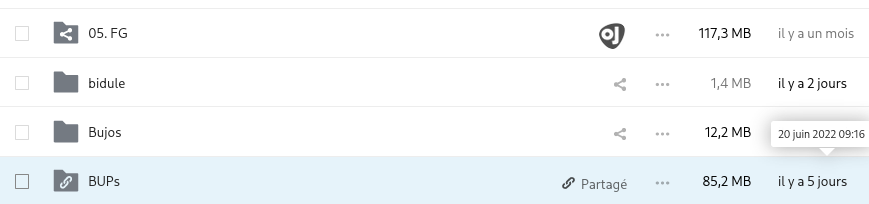
\includegraphics{./Captures/nuage.partager.icones.png}
	\caption{Deux exemples de ressources partagées et deux autres non partagées.}
\end{figure}
Ainsi, le dossier \og~O5 FG~\fg{} a été utilisé par un autre utilisateur dont les initiales sont OJ (puisqu'aucun avatar ne semble avoir été défini par l'utilisateur). 
Le dossier \og~BUPs~\fg{} par contre fait l'objet d'un partage de ma part. 
Il est intéressant de noter que les icônes représentant ces deux ressources et les deux autres (Bidule et Bujos) diffèrent et que suivant le sens du partage le motif superposé à l'icône n'est pas le même. 

\subsection{Les options de partage avancées}
%\addcontentsline{toc}{subsection}{Les options du partage}
Pour avoir  plus de détails il suffit soit de cliquer sur l'icône \ldots soit sur l'icône de partage et alors le volet latéral des propriétés de partage apparaîtra.
\begin{figure}
	\centering
	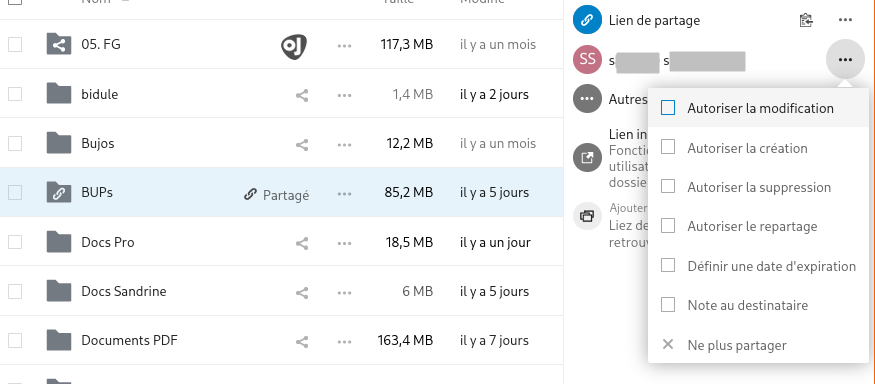
\includegraphics{./Captures/nuage.partager.menu.contextuel.png}
	\caption{Les différentes possibilités de partage offertes.}
\end{figure}

On voit par la dernière capture qu'il est possible de gérer les droits de modification, de création ou de suppression sur la ressource, mais aussi d'autoriser le repartage et, plus intéressant encore, de définir un mot de passe d'accès et une date d'expiration du partage.